\newpage
\subsection{Caso d'uso UC9 - Acquisto API}
\label{UC9}
\begin{figure}[ht]
	\centering
	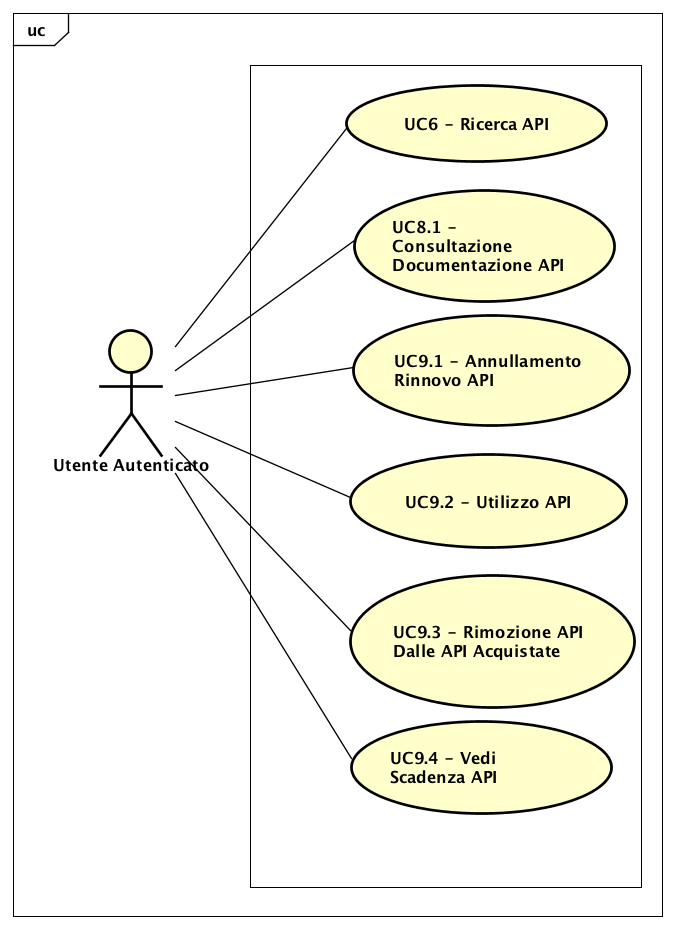
\includegraphics[scale=0.45]{UML/UC9.png}
	\caption{UC9: Visualizzazione API registrate}
\end{figure}

\begin{longtable}{ l | p{11cm}}
	\hline
	\rowcolor{Gray}
	\multicolumn{2}{c}{UC9 - Acquisto API}\\
	\hline
	
	 \textbf{Attori} & Utente autenticato  \\
	\textbf{Descrizione} & L'attore può effettuare l'acquisto dell'API selezionata tramite i crediti da lui posseduti \\
	\textbf{Pre-Condizioni} & L'attore seleziona il pulsante relativo all'acquisto dalla pagina della singola API  \\
	\textbf{Post-Condizioni} & L'attore visualizza la pagina per poter effettuare l'acquisto\\
	\textbf{Scenario Principale} & 
	\begin{enumerate*}[label=(\arabic*.),itemjoin={\newline}]
		\item L'attore visualizza il nome dell'API (UC7.1)
		\item L'attore visualizza l'autore dell'API (UC7.3)
		\item L'attore visualizza un menù per la scelta della licenza da acquistare (UC9.1)
		\item L'attore visualizza il saldo disponibile nel suo portafoglio virtuale (UC????)
		\item L'attore visualizza il prezzo dell'API selezionata (UC7.8)
		\item L'attore visualizza il saldo preventivato in seguito all'acquisto della licenza selezionata (UC9.2)
		\item L'attore può confermare l'acquisto qualora abbia crediti sufficienti, e venire reindirizzato ad una schermata di riepilogo (UC9.3)
	\end{enumerate*}\\
	\textbf{Scenari Alternativi} & 
	\begin{enumerate*}[label=(\arabic*.),itemjoin={\newline}]
		\item L'attore visualizza un apposito pulsante per poter ricaricare i propri crediti (tramite opportuna pagina) qualora essi non siano sufficienti a completare la transazione (UC9.4)
		\item L'attore visualizza un messaggio ad indicare che la transazione non è andata a buon fine, per motivi differenti dal proprio saldo (UC9.5)
	\end{enumerate*}\\
\end{longtable}


\subsubsection{Caso d'uso UC9.1: Visualizzazione menù licenza}
\label{UC9_1}

\begin{minipage}{\linewidth}
	\begin{tabular}{ l | p{11cm}}
		\hline
		\rowcolor{Gray}
		\multicolumn{2}{c}{UC9.1 - Visualizzazione menù licenza} \\
		\hline
		\textbf{Attori} & Utente autenticato \\
		\textbf{Descrizione} & L'attore visualizza un menù relativo alla scelta della licenza da acquistare e può effettuare la scelta più consona secondo il proprio interesse\\
		\textbf{Pre-Condizioni} & L'attore visualizza il menù per la scelta della licenza\\
		\textbf{Post-Condizioni} & L'attore ha selezionato la licenza a lui più consona, oppure accetta la scelta di default \\
		\textbf{Scenario Principale} & 
		\begin{enumerate*}[label=(\arabic*.),itemjoin={\newline}]
			\item L'attore può selezionare la licenza più consona alle sue necessità, tra quelle rese disponibili dall'autore, tramite il menù preposto
		\end{enumerate*}\\
		\textbf{Scenari Alternativi} & 
		\begin{enumerate*}[label=(\arabic*.),itemjoin={\newline}]
			\item L'attore non modifica la scelta di default, accettandola
		\end{enumerate*}\\
	\end{tabular}
\end{minipage}

\subsubsection{Caso d'uso UC9.2: Previsione saldo}
\label{UC9_2}

\begin{minipage}{\linewidth}
	\begin{tabular}{ l | p{11cm}}
		\hline
		\rowcolor{Gray}
		\multicolumn{2}{c}{UC9.2 - Previsione saldo} \\
		\hline
		\textbf{Attori} & Utente autenticato \\
		\textbf{Descrizione} & L'attore visualizza una previsione del proprio saldo crediti in seguito all'acquisto\\
		\textbf{Pre-Condizioni} & L'attore si trova nella pagina preposta all'acquisto di un'API\\
		\textbf{Post-Condizioni} & L'attore visualizza una previsione del proprio saldo in seguito all'acquisto \\
		\textbf{Scenario Principale} & 
		\begin{enumerate*}[label=(\arabic*.),itemjoin={\newline}]
			\item L'attore può visualizzare una previsione del proprio saldo qualora portasse a termine l'acquisto della licenza selezionata nel caso d'uso UC9.1
		\end{enumerate*}\\
	\end{tabular}
\end{minipage}

\paragraph{Caso d'uso UC9.3: Riepilogo acquisto}
\label{UC9_3}

\begin{minipage}{\linewidth}
	\begin{tabular}{ l | p{11cm}}
		\hline
		\rowcolor{Gray}
		\multicolumn{2}{c}{UC9.3 - Riepilogo acquisto} \\
		\hline
		\textbf{Attori} & Utente autenticato \\
		\textbf{Descrizione} & L'attore visualizza un riepilogo dell'acquisto appena effettuato\\
		\textbf{Pre-Condizioni} & L'attore ha confermato l'acquisto per un API\\
		\textbf{Post-Condizioni} & L'attore visualizza un messaggio di conferma e la chiave per l'API, che verrà inviata anche tramite email dal sistema\\
		\textbf{Scenario Principale} & 
		\begin{enumerate*}[label=(\arabic*.),itemjoin={\newline}]
			\item L'attore può visualizzare un messaggio di ringraziamento e riepilogo per l'acquisto effettuato.
			\item L'attore può visualizzare l'API key relativa all'acquisto andato a buon fine (UC7.8)
		\end{enumerate*}\\
	\end{tabular}
\end{minipage}

\paragraph{Caso d'uso UC9.4: Pulsante saldo insufficiente}
\label{UC9_4}

\begin{minipage}{\linewidth}
	\begin{tabular}{ l | p{11cm}}
		\hline
		\rowcolor{Gray}
		\multicolumn{2}{c}{UC9.4 - Pulsante saldo insufficiente} \\
		\hline
		\textbf{Attori} & Utente autenticato \\
		\textbf{Descrizione} & L'attore visualizza il pulsante per poter ricaricare il proprio saldo\\
		\textbf{Pre-Condizioni} & L'attore ha confermato l'acquisto per un API, ma non possiede un saldo sufficiente\\
		\textbf{Post-Condizioni} & L'attore visualizza un pulsante per essere reindirizzato alla pagina preposta alla ricarica dei crediti\\
		\textbf{Scenario Principale} & 
		\begin{enumerate*}[label=(\arabic*.),itemjoin={\newline}]
			\item L'attore può selezionare il pulsante ed essere reindirizzato alla pagina preposta alla ricarica dei crediti personali (UC????)
		\end{enumerate*}\\
	\end{tabular}
\end{minipage}

\paragraph{Caso d'uso UC9.5: Errore acquisto}
\label{UC9_5}

\begin{minipage}{\linewidth}
	\begin{tabular}{ l | p{11cm}}
		\hline
		\rowcolor{Gray}
		\multicolumn{2}{c}{UC9.5 - Errore acquisto} \\
		\hline
		\textbf{Attori} & Utente autenticato \\
		\textbf{Descrizione} & L'attore visualizza un errore relativo all'acquisto, non correlato al proprio saldo personale\\
		\textbf{Pre-Condizioni} & L'attore ha confermato l'acquisto per un API, si è verificato un errore\\
		\textbf{Post-Condizioni} & L'attore visualizza un errore relativo all'acquisto, con opportuna descrizione\\
		\textbf{Scenario Principale} & 
		\begin{enumerate*}[label=(\arabic*.),itemjoin={\newline}]
			\item L'attore può visualizzare un errore relativo all'acquisto, non inerente al proprio saldo, con opportuna descrizione
		\end{enumerate*}\\
	\end{tabular}
\end{minipage}
